\documentclass[12pt,a4paper]{scrartcl}
\usepackage[utf8]{inputenc}
\usepackage{mathtools}
\usepackage[english,russian]{babel}
\usepackage{indentfirst}
\usepackage{misccorr}
\usepackage{amsmath}
\usepackage{mathptmx}
\usepackage{physics}

\usepackage{graphicx}

\usepackage[rightcaption]{sidecap}
\usepackage{wrapfig}

\begin{document}
\begin{titlepage}
  \begin{center}
     
    \vspace{0.5cm}
 
    НОВОСИБИРСКИЙ ГОСУДАРСТВЕННЫЙ УНИВЕРСИТЕТ
    \vspace{0.25cm}
     
    Механико-математический факультет
     
    Кафедра: Математика и компьютерные науки
    \vfill
     
     
    Тлепбергенова Дарья Дулатовна
    \vfill
 
    \textsc{Отчет по вычислительному практикуму}\\[5mm]
     
    {\LARGE Решение уравнения теплопроводности\\
      с помощью неявного метода Эйлера.\\
    Вариант 12.\\[2mm]}
  \bigskip
     
    3 курс, группа 16121
\end{center}
\vfill
 \newlength{\ML}
\settowidth{\ML}{«\underline{\hspace{0.7cm}}» \underline{\hspace{2cm}}}
\hfill\begin{minipage}{0.4\textwidth}
  Преподаватель:\\
  Махоткин Олег Александрович
\end{minipage}%
\bigskip

 \vfill
\begin{center}
  Новосибирск, 2018 г.
\end{center}
\end{titlepage}

\newpage
\section{Постановка задачи.}
Дано уравнение теплопроводности в виде:
\begin{align}\label{main}
    \begin{cases}
        \frac{\partial u}{\partial t} = a^{2}
        {\dfrac{{\partial}^2 u}{\partial x^{2}}}+f(x,t) \\
        0\le x \le 1, 0\le t \le1 \\
        u(x,0) = \mu(x) \\
        u(0,t) = \mu_1(t) \\
        u(1,t) = \mu_2(t) \\
    \end{cases}
\end{align}
Для $\mu(x) = -4x^{4}+2x^{2}$,$ \\
    \mu_1(t) = t^{2}-t$,$ \\
    \mu_2(t) = 1+t+t^{2}-t e^{x}$,$ \\
    f(x,t) = x+2 t-e^{x}+a(12 x^{2}-4+t e^{x}) $,$\\
    u(x,t) = -x^{4}+2 x^{2}+t x+t^{2}-t e^{x} $,$\\
    a = 0.021 $\\

Выполнить следующие пункты:
\begin{enumerate}
    \item Исследовать данную схему на точность и устойчивость.
    \item Проверить, что $u(x,t)$ является решением краевой задачи.
    \item Написать программу для решения уравнения теплопроводности методом конечных разностей.
    \item Выводить на экран значения относительной погрешности разностного решения в заданных контрольных точках по $t$. Использовать любую из трех основных норм вектора.
\end{enumerate}
\section{Описание вычислительного метода.}
Перейдем к дискретной постановке задачи: разобьем наши промежутки по $x$ и по $t$ на $N_x$ и $N_t$ равных частей соответственно. Получим систему:

\begin{align}
    \begin{cases}
        &\frac{u^{j+1}_k-u^{j}_k}{\tau} = a^{2} \frac{u^{j+1}_{k+1}-2 u^{j+1}_k+u^{j+1}_{k-1}}{h^{2}}+f^{j+1}_k\\
        &\Bigl\{x_k = k h $ : $ h = \frac {1}{N_x}, k = 0 ..N_x\Bigr\}\\
        &\Bigl\{t_j = j \tau $ : $ \tau =\frac {1}{N_t}, j = 0 ..N_t \Bigr\}\\ \label{dis}
        &u^{0}_k = \mu(x_k) \\
        &u^{t}_0 = \mu_1(t_j) \\
        &u^{t}_{N_{x}} = \mu_2(t_j) \\ 
    \end{cases}
\end{align}

\section{Исследование данной схемы на точность и устойчивость.}
Погрешность аппроксимации:
\begin{align*}
    \psi^{j}_k = f(x_i,t_{n+1}) - \frac{u(x_k,t_{j+1}-u(x_k,t_j)}{\tau}+a \frac{u(x_{k+1},t_{j+1}) - 2 u(x_k,t_{j+1})+u(x_{k-1},t_{j+1})}{h^{2}} = \\
\end{align*}
Разложим в Ряд Тейлора в $x_i$, где $t$'$ \in [t_j,t_{j+1}]$:
\[
=f- \pdv{u}{t}+ \frac{\tau}{2}\pdv[2]{u}{t}(x_{i},t^{'})+a \pdv[2]{u}{x}+ \frac{a^{2} h^{2}}{24}(\pdv[4]{u}{x}(x^{-},t_{j+1})+\pdv[4]{u}{x}(x^{+},t_{j+1})) = O(\tau+h^{2})\\   
\]
Погрешность решения:
\begin{align*}
    L_{\tau,h} \xi^{\tau,h} &= \psi^{\tau,h}\\
    \xi^{j}_{k} &= u^{j}_k - u(x_k,t_j) \\
    (1+ \frac{2 a^{2} \tau}{h^{2}}) \xi^{j+1}_{k} &= \xi^{j}_{k}+ \frac{a^{2} \tau}{h^{2}} (\xi^{j+1}_{k-1}+\xi^{j+1}_{k+1}) +\tau \psi^{j}_k\\
\end{align*}
Возьмем модуль:
\begin{align*}
    (1+ \frac{2 a^{2} \tau}{h^{2}})| \xi^{j+1}_{k}|  \le |\xi^{j}_{k}|+ \frac{a^{2} \tau}{h^{2}} (|\xi^{j+1}_{k-1}|+|\xi^{j+1}_{k+1}|) +\tau |\psi^{j}_k | \le\\
    \le \max_{k=0..N_{x}} |\xi^{j}_{k}|+ \frac{a^{2} \tau}{h^{2}} (\max_{k=0..N_{x}}|\xi^{j+1}_{k-1}|+\max_{k=0..N_{x}}|\xi^{j+1}_{k+1}|) +\tau \max_{k,j=0..N_{x},N_{t}}|\psi^{j}_k|\\
\end{align*}
Обозначим через $\delta^{j} = \max_{k=0..N_{x}} |\xi^{j}_{k}|$получим неравенство:
\begin{align*}
    \delta^{j} \le \delta^{j+1}+\tau \max_{k,j=0..N_{x},N_{t}}|\psi^{j}_k| \\
\end{align*}
Учитывая то, что $\delta^{0} = \max_{k=0..N_{x}} \mu(x_k)$ получаем:
\begin{align*}
    \delta^j \le \max_{k=0..N_{x}} \mu(x_k) + j \tau \max_{k,j=0..N_{x},N_{t}}|\psi^{j}_k| \\
    \Rightarrow \max_{k=0..N_{x}} |\xi^{j}_{k}| = O(\tau + h^{2})
\end{align*}
\section{Проверим, что $u(x,t)$ - решение системы.}
Подставим в систему \eqref{main}:
\begin{align*}
    \frac{\partial u}{\partial t} &= x+ 2 t -e^{x} = a(-12 x^{2} + 4 - t e^{x}) + x+ 2 t - e^{x} + a(12 x^{2} - 4 +t e^{x}) \\
    \frac{\partial u}{\partial t} &= -4 x^{3} +4 x+t-t e^{x} 
\end{align*}
Проверим краевые условия:
\begin{align*}
    u(x,0) &= - x^{4}+2 x^{2} = \mu(x) \\
    u(0,t) &= t^{2}-t = \mu_1(t) \\
    u(1,t) &= -1+2+t+t^{2}-t e = \mu_2(t) \\
\end{align*}
Значит функция $u(x,t)$ является решением системы \eqref{main}
\section{Описание алгорима.}
\begin{itemize}
    \item Main class 
    \begin{itemize}
        \item Создаем поля для разбиения сетки, коэффициента для
        второй производной (main class для простоты замены начальных
        данных)
        \item Создаем функции краевых условий и решения (main class
        для простоты замены начальных данных)
        \item В main функции обращаемся к методу решения уравнения
        теплопроводности и запускаем визуализацию на питоне сначала
        для
        решения, потом для точного решения
    \end{itemize}
    \item HeatEquation class
    \begin{itemize}
        \item создаем поле аналога числа Куранта (для упрощения
        формул
        вычислений)
        \item создаем поля для шага по $t,x$  
        \item функция для решения уравнения теплопроводности:
        \begin{itemize}
            \item создаем двумерный массив для записи решения 
            \item заполняем его первую строку и первый и последний 
            столбец начальными значениями
            \item для оставшихся строк решение находится построчно 
            методом прогонки через предыдущее:
            \item функция метода прогонки с постоянными
            коэффициентами:
            \begin{itemize}
                \item в данном случае диагональные элементы одинаковы
                и над/поддиагональные тоже, по этому заводим для них
                2 переменные
                \item также заводим два массива из метода прогонки и 
                находим для них коэффициенты с последнего до первого
                (в силу диагонального преобладания)
                \item далее находим координаты искомого вектора, начиная с первого.
                \item возвращаем этот вектор.
            \end{itemize}
            \item после нахождения всех коэффициентов матрицы
            решений, записываем ее в текстовый файл для графического
            вывода, подсчитываем максимальную ошибку (через
            максимум модуля) и печатаем ее.
        \end{itemize}
    \end{itemize}
\end{itemize}
\section{Код программы (на Java).}
\subsection{Класс HeatEquation}
\begin{verbatim}
package ru.nsu.mmf.g16121.ddt.math;

import java.io.FileNotFoundException;
import java.io.PrintWriter;

import static ru.nsu.mmf.g16121.ddt.main.Main.*;

public class HeatEquations {

    private static final double stepX = (rightBound - leftBound) /
            NUMBERS_COUNT_OF_GRID_BY_X;
    private static final double stepT = (rightBound - leftBound) /
            NUMBERS_COUNT_OF_GRID_BY_T;

    private static final double COURANT_NUMBER_ANALOGUE =
            2.0 * COEFFICIENT_AT_SECOND_DERIVATIVE * stepT /
            Math.pow(stepX, 2);

    /**
     * @param rightPart - this is array of the right part of linear
     *                  equation system Au = rightPart, where A is
     *                  triDiagonal matrix with coeff:
     *                  diag - is coefficient of the matrix A on the 
     *                  diagonal;
     *                  overDiagonal - the coefficient of the matrix
     *                  And the overdiagonal and subdiagonal;
     *                  <p>
     * @return solution matrix of a linear system.
     */

    private static double[] sweepMethodWithConstCoef(
    double[] rightPart) {
        double diag = 1.0 + COURANT_NUMBER_ANALOGUE;
        double overDiagonal = -COURANT_NUMBER_ANALOGUE * 0.5;

        double[] u = new double[rightPart.length];

        double[] alpha = new double[rightPart.length - 1];
        double[] beta = new double[rightPart.length - 1];

        alpha[rightPart.length - 2] = -overDiagonal / diag;
        beta[rightPart.length - 2] = rightPart[rightPart.length - 1] /
        diag;

        for (int i = rightPart.length - 3; i >= 0; i--) {
            alpha[i] = -(overDiagonal / (diag + overDiagonal * 
            alpha[i + 1]));
            beta[i] = ((rightPart[i + 1] - beta[i + 1] * overDiagonal)
            /(diag + overDiagonal * alpha[i + 1]));
        }

        u[0] = ((rightPart[0] - overDiagonal * beta[0]) / (diag +
                overDiagonal * alpha[0]));
        for (int i = 1; i < rightPart.length; i++) {
            u[i] = alpha[i - 1] * u[i - 1] + beta[i - 1];
        }
        return u;
    }

    /**
     * Tn this method (<>writeInTxt</>) we write points surface in 
     * txt file: x - in 1st column, t - in 2d column,
     * exact value of the func - 3d column and our func value in 
     * 4d column (for gnuplot)
     */

    private static void writeForGnuplot(double[][] u) throws
    FileNotFoundException {
        PrintWriter writer = new
        PrintWriter("functions_for_Gnuplot.txt");

        double x;
        double t = leftBound;
        for (int i = 0; i <= NUMBERS_COUNT_OF_GRID_BY_T; i++) {
            x = leftBound;
            for (int j = 0; j <= NUMBERS_COUNT_OF_GRID_BY_X; j++) {
                writer.println(x + "\t" + t + "\t" + u(x, t) + "\t" 
                + u[i][j]);
                x += stepX;
            }
            t += stepT;
        }
        writer.close();
    }

    private static void writeResultForPython(double[][] u) throws
    FileNotFoundException {
        PrintWriter writer = new PrintWriter("result.txt");

        writer.print("[[" + (int) leftBound + ", " + (int) rightBound
                + ", " + (NUMBERS_COUNT_OF_GRID_BY_X + 1) + "],");
        writer.print("[" + (int) leftBound + ", " + (int) rightBound
                + ", " + (NUMBERS_COUNT_OF_GRID_BY_T + 1) + "],");

        double x;
        double t = leftBound;

        writer.print("[");
        for (int i = 0; i <= NUMBERS_COUNT_OF_GRID_BY_T; i++) {
            x = leftBound;
            writer.print("[");
            for (int j = 0; j < NUMBERS_COUNT_OF_GRID_BY_X; j++) {
                writer.print(u[i][j] + ",");
                x += stepX;
            }
            writer.print(u[i][NUMBERS_COUNT_OF_GRID_BY_X]);
            if (i == NUMBERS_COUNT_OF_GRID_BY_T) {
                writer.print("]");
            } else {
                writer.print("],");
            }
            t += stepT;
        }
        writer.print("]]");
        writer.close();
    }

    private static void writeMainFuncForPython() throws
    FileNotFoundException {
        PrintWriter writer = new PrintWriter("mainFunc.txt");

        writer.print("[[" + (int) leftBound + ", " + (int) rightBound
                + ", " + (NUMBERS_COUNT_OF_GRID_BY_X + 1) + "],");
        writer.print("[" + (int) leftBound + ", " + (int) rightBound
                + ", " + (NUMBERS_COUNT_OF_GRID_BY_T + 1) + "],");

        double x;
        double t = leftBound;

        writer.print("[");
        for (int i = 0; i <= NUMBERS_COUNT_OF_GRID_BY_T; i++) {
            x = leftBound;
            writer.print("[");
            for (int j = 0; j < NUMBERS_COUNT_OF_GRID_BY_X; j++) {
                writer.print(u(x, t) + ",");
                x += stepX;
            }
            writer.print(u(x, t));
            if (i == NUMBERS_COUNT_OF_GRID_BY_T) {
                writer.print("]");
            } else {
                writer.print("],");
            }
            t += stepT;
        }
        writer.print("]]");
        writer.close();
    }

    private static double maxError(double[][] u) {

        double x = leftBound;
        double t = leftBound;
        double max = Math.abs(u[0][0] - u(x, t));
        for (int i = 0; i <= NUMBERS_COUNT_OF_GRID_BY_T; i++) {
            x = leftBound;
            for (int j = 0; j <= NUMBERS_COUNT_OF_GRID_BY_X; j++) {
                double error = Math.abs(u(x, t) - u[i][j]);
                if (error > max) {
                    max = error;
                }
                x += stepX;
            }
            t += stepT;
        }
        return max;
    }

    /**
     * Tn this method (<>solveHeatEquation</>) solve the heat
     * equation solves the heat equation using the Euler method,
     * with initial conditions, and writes data to a text file 
     * to display the result.
     */

    public static void solveHeatEquation() 
    throws FileNotFoundException {
        double[][] u = new double[NUMBERS_COUNT_OF_GRID_BY_T + 1]
                [NUMBERS_COUNT_OF_GRID_BY_X + 1];

        //The first row of the matrix is filled by the initial data.
        double x = leftBound;
        for (int i = 0; i <= NUMBERS_COUNT_OF_GRID_BY_X; i++) {
            u[0][i] = mu(x);
            x += stepX;
        }

        //The first and second columns are filled with source data.
        double t = leftBound;
        for (int j = 0; j <= NUMBERS_COUNT_OF_GRID_BY_T; j++) {
            u[j][0] = mu1(t);
            u[j][NUMBERS_COUNT_OF_GRID_BY_X] = mu2(t);
            t += stepT;
        }

        //build the right part for the sweep method
        t = leftBound;
        for (int j = 0; j <= NUMBERS_COUNT_OF_GRID_BY_T - 1; j++) {
            x = leftBound + stepX;
            double[] rightPart = 
            new double[NUMBERS_COUNT_OF_GRID_BY_X - 1];
            for (int i = 0; i <= NUMBERS_COUNT_OF_GRID_BY_X - 2; i++) {
                rightPart[i] = u[j][i + 1] + stepT * f(x, t + stepT);
                x += stepX;
            }
            rightPart[0] += COURANT_NUMBER_ANALOGUE * 0.5 * 
            mu1(t + stepT);
            rightPart[NUMBERS_COUNT_OF_GRID_BY_X - 2] +=
            COURANT_NUMBER_ANALOGUE * 0.5 * mu2(t + stepT);

            //fill the rest of the matrix
            System.arraycopy(sweepMethodWithConstCoef(rightPart),
                    0, u[j + 1], 1, NUMBERS_COUNT_OF_GRID_BY_X - 1);
            t += stepT;
        }

        //write in the txt for display the result
        writeForGnuplot(u);
        writeMainFuncForPython();
        writeResultForPython(u);
        System.out.println("Max error = " + maxError(u));
    }
}
\end{verbatim}
\subsection{Класс  Main}
\begin{verbatim}
package ru.nsu.mmf.g16121.ddt.main;

import ru.nsu.mmf.g16121.ddt.math.HeatEquations;

import java.io.IOException;

public class Main {
    public static final double leftBound = 0;
    public static final double rightBound = 1;

    public static final int NUMBERS_COUNT_OF_GRID_BY_X = 10;
    public static final int NUMBERS_COUNT_OF_GRID_BY_T = 20;

    public static final double 
            COEFFICIENT_AT_SECOND_DERIVATIVE = 0.021;

    public static double f(double x, double t) {
        return (x + 2.0 * t - Math.exp(x) + 
                COEFFICIENT_AT_SECOND_DERIVATIVE * (12.0 * 
                        Math.pow(x, 2) - 4.0 + t * Math.exp(x)));
    }

    public static double mu(double x) {
        return -Math.pow(x, 4) + 2.0 * Math.pow(x, 2);
    }

    public static double mu1(double t) {
        
        return Math.pow(t, 2) - t;
    }

    public static double mu2(double t) {
        return 1 + t + Math.pow(t, 2) - t * Math.E;
    }

    public static double u(double x, double t) {
        return -Math.pow(x, 4) + 2.0 * Math.pow(x, 2) 
                + t * x + Math.pow(t, 2) - t * Math.exp(x);
    }

    public static void main(String[] args) throws IOException {
        HeatEquations.solveHeatEquation();

        Runtime.getRuntime().exec("python3 vizualization.py");
        Runtime.getRuntime().exec("python3 vizualization2.py");
    }
}

\end{verbatim}
  \newpage  

\section{Графический вывод (Тесты)}
При $h = 5$ и $\tau = 5$ 
\begin{figure}[h]
    \centering
    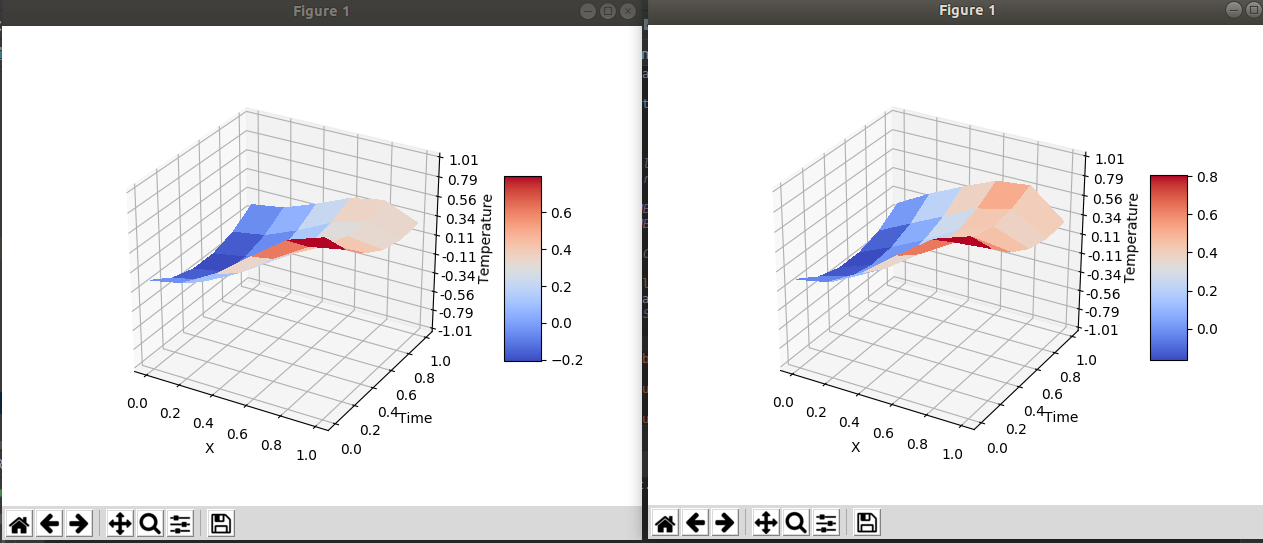
\includegraphics[width=14cm]{t5h5.png}
    \caption{Слева - решение системы неявным методом Эйлера,
                справа - точное решение}
\end{figure}
\\
Тогда максимальная ошибка: 
\begin{figure}[h]
    \centering
    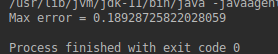
\includegraphics[width=6cm]{error1.PNG}
\end{figure}
\\
Теперь увеличим $h$ в 2 раза, а $\tau$ в 4 раза: \\
При $h = 10$ и $\tau = 20$:
\begin{figure}[h]
    \centering
    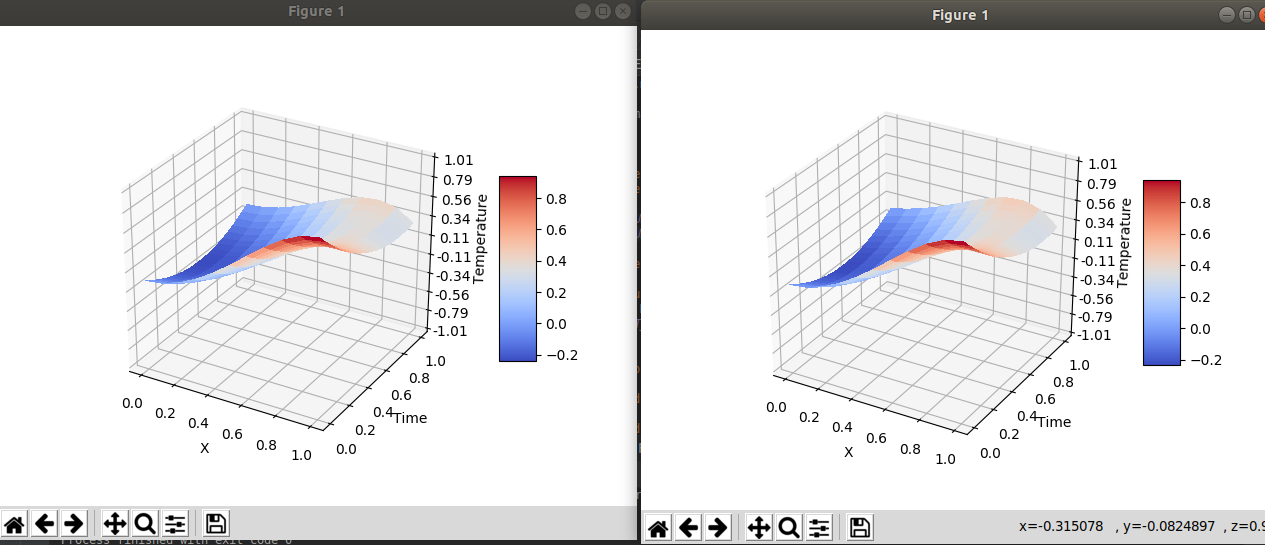
\includegraphics[width=14cm]{t20h10.png}
    \caption{Слева - решение системы неявным методом Эйлера,
                справа - точное решение}
\end{figure}
\\
Тогда максимальная ошибка должна уменьшится в 4 раза: а по факту уменьшилась примерно 3,9 раз \\
\begin{figure}[h]
    \centering
    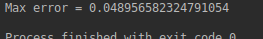
\includegraphics[width=6cm]{error2.png}
\end{figure}
\\
Теперь выберем большие $h,\tau$, чтобы убедиться в том, что поверхности совпадут: \\
При $h = 500$ и $\tau = 500$ \\
\begin{figure}[h]
    \centering
    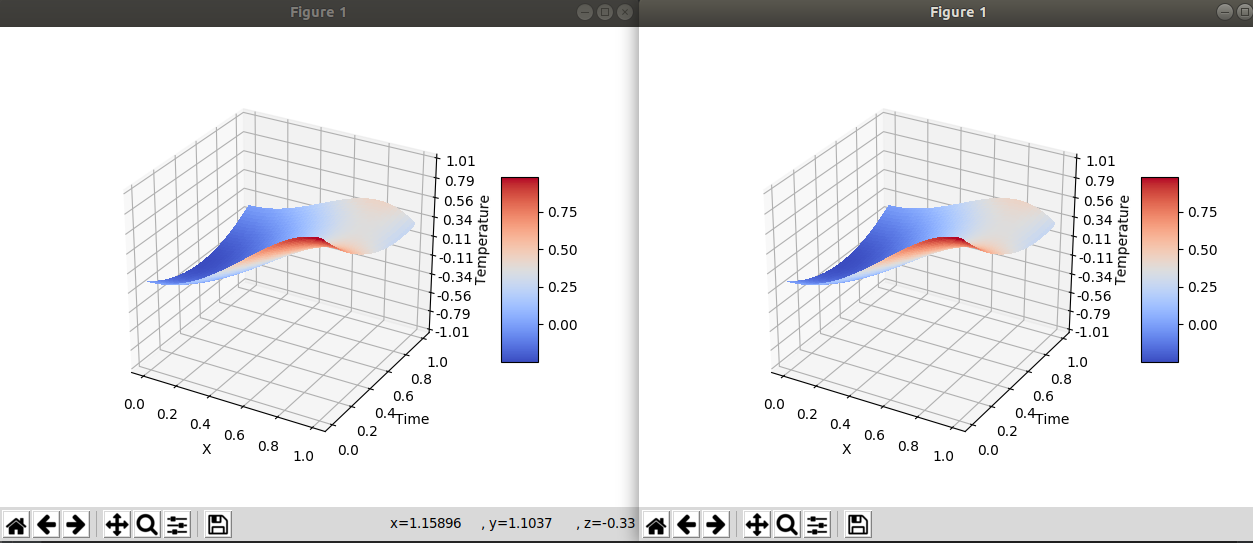
\includegraphics[width=14cm]{t500h500.png}
    \caption{Слева - решение системы неявным методом Эйлера,
                справа - точное решение}
\end{figure}
\\
Как видно на рисунке, графики практически идентичны и почти непрерывны для человеческого взгляда.

\section{Выводы.}
Таким образом мы установили, что неявный метод Эйлера является устойчивым, и не зависит от $\tau,h$ или $a$ как, например, явный метод Эйлера, но, с другой стороны при малых $\tau, h$ погрешность решения достаточно велика и, следовательно, решение не достаточно точное.

Также убедились на практике, что данный метод при достаточно больших $\tau, h$ наше дискретное решение практически не отличимо от непрерывного, что значительно упрощает решения многих видов уравнений.

Мы увидели, что теоретическая погрешность, которую мы посчитали до прогонки решения, практически совпадает с действительной погрешностью, а значит мы можем выбрать нужную нам точность решения заранее, что не мало важно для методов вычислений.
\end{document}


